\documentclass{beamer}

\usepackage[english]{babel}
\usepackage[utf8]{inputenc}
\usepackage{lmodern}% http://ctan.org/pkg/lm
%\usepackage{times} %font
\usepackage{amsmath, amsthm, amssymb}
%\boldmath
\usepackage{fontawesome, ragged2e}
\usepackage[backend=biber, style=nature, natbib=true, date=year, sorting=ynt, doi=false,isbn=false,url=false,eprint=false, maxbibnames=1]{biblatex} 
\AtEveryBibitem{\clearfield{pages}} 
\addbibresource{references.bib}
\usetheme{Custom} % beamerThemeCustom.sty
\usepackage[orientation=portrait,size=a0,scale=1]{beamerposter}
\usepackage{csquotes}
\usepackage{booktabs}
\usepackage{siunitx}
\usepackage{caption}


% Make the figure caption labels bold
%\setbeamerfont{caption}{series=\bfseries}
% Beamer disables figure numbering by default (it assumes figure numbers on slides would not make sense). This command restores autonumbering
%\setbeamertemplate{caption}[numbered]
%\setbeamerfont{caption name}{series=\bfseries}
%\setbeamertemplate{caption label separator}[period]

\title{Planned Master Thesis: \\[1ex] Austrian Beekeeper Citizens Science Survey, the Financial Burden to Fight \textit{Varroa Destructor}}
\author[\faEnvelope{} hoberreiter@gmail.com \faTwitter{} @btree\_hannes]{Hannes Oberreiter}
\institute
{University Graz, Institut of Biology}
\date{\today}
\logo{
\includegraphics[height=5.5cm]{img/logo_uni_graz_4c.jpg}}

\begin{document}
\begin{frame}{} 

%%%%%%%%%%%%%
% 1. Row %%%%
%%%%%%%%%%%%%
\begin{columns}[t]
  %%%%%%%%%%%%%
  % 1. Col %%%%
  %%%%%%%%%%%%%
  \begin{column}{0.49\textwidth}

    \begin{block}{Introduction}
      %\begin{minipage}[t][30cm][c]{0.97\textwidth} \vskip-\baselineskip
      Our planned research deals with beekeeping in Austria and the expenses involved in the use of medication against the parasitic mite \textit{Varroa destructor}. In the foreground of the work is an exploratory analysis of a citizen science survey data from the years 2018/19 and 2019/20. The survey is carried out since 2008 by the Institute of Biology at the University of Graz to collect data on winter losses of bee colonies \citep{brodschneider2013}. In the past two years the participants could also answers a question about the costs of treatment per bee colony. \\
      Such a descriptive analysis of treatment expenses has never been carried out in Austria in this form before. However, the data could clearly show how great the economic burden for beekeeping, caused by the introduced aggressor, is and could yield valuable information about the dimensions of the Austrian treatment agent market. \\
      Secondly, I would like to deal with the hypothesis whether there is a connection between the amount of costs used for control and the loss rates of bee colonies in winter. Since different methods are not always equally successful in treatment \citep{brodschneider2013, crailsheim2018, oberreiter2020} and probably also cause different expenses, the expenditure per colony could mean a direct correlation with the winter colony losses for the beekeeper. Additionally higher losses mean additional costs for the beekeeping business.
      \begin{figure}
      \centering
      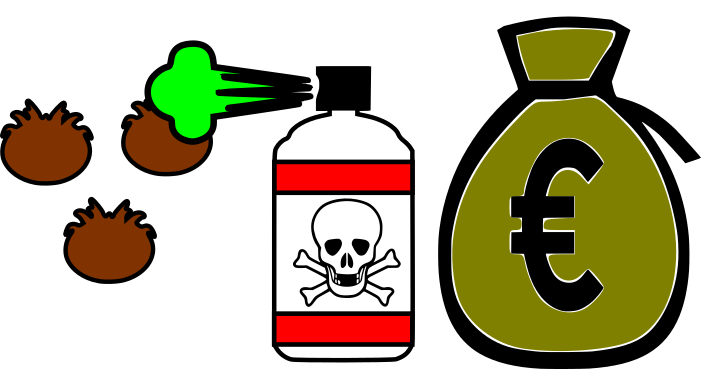
\includegraphics[width=.7\textwidth]{img/drawing.png}
      \end{figure}
      %\end{minipage}
    \end{block}

    \begin{block}{Material and Methods}
      %\begin{minipage}[t][0.15\paperheight][c]{0.97\textwidth} \vskip-\baselineskip
      The survey consisted of question from the international COLOSS questionnaire and some additional questions which were only present in the Austrian survey. Our main interest in this study are the surveyed questions about the \enquote{Estimated Costs of Treatment against Varroa Mites per Colony}, the number of colonies wintered, number of colonies lost (without natural disasters) and the methods and application time of varroa control. \\
      Data validation and error control was performed with logical operators. We excluded responses which did answers treatment costs but did no treatment against Varroa mites ($n=3$). Zero costs answers which were unplausible ($n=19$) or got a sponsorship ($n=4$) (e.g. local community) were also removed. Some Participants did answers with a very high costs per colony, after further investigations we found out that most did answer not cost per colony but gave their total expenses per operation and therefore the costs were divided by the number of colonies wintered ($n=118$). \\
      Statistical analysis is performed with R and for full reproducibility we want also to publish the source on Github and as Docker Container after the results are published. Categorical predictor variables are compared with ANOVA and by significant difference ($p<0.05$) followed with $p$-value family-wise error corrected (Holm, Step Down) pairwise t-test. Loss rates estimations and corresponding confidence intervalls, which are not yet done, will be computed with a quasibinominal generalized linear model (GZLM) link \enquote{logit} function \citep{vanderzee2013}. \\
      Both survey years are analysed separately as we do not know if the survey participants are independent, because of the anaonym design of the questionnaire.
      %\end{minipage}
    \end{block}

    \begin{block}{Descriptive Statistics}
      \begin{minipage}[t][40cm][c]{0.97\textwidth} 
      \begin{table}
      \caption{Number of participants answering the question for estimated cost per colony in the survey for both survey years, compared to total participants.}
      \begin{tabular}[]{l*{2}{c}S[table-format=2.1]}
      \toprule
      Year & {Total {[}$n${]}} & {Answered {[}$n${]}} & {Percent {[}\%{]}} \tabularnewline
      \midrule
      18/19 & 1534 & 1195 & 77.9\tabularnewline
      19/20 & 1539 & 1170 & 76.0\tabularnewline
      \bottomrule
      \end{tabular}
      \end{table}
      \begin{table}
      \centering
      \caption{Descriptive statistics of expenses and estimates, based on our own estimation of expenses, in Euro. Both survey years are together.}
      \begin{tabular}[]{l*{6}{S[table-format=4.4]}}
      \toprule
      Type & {Minimum} & {1. Quantile} & {Median} & {Mean} & {3. Quantile} & {Maximum}\tabularnewline
      \midrule
      Survey & 0.00 & 5.00 & 8.33 & 9.98 & 12.50 & 250.00 \tabularnewline
      Estimated & 0.00 & 8.05 & 10.65 & 12.18 & 14.02 & 167.32 \tabularnewline
      \bottomrule
      \end{tabular}
      \end{table}
      \vspace{3cm}
      \begin{figure}
      \centering
      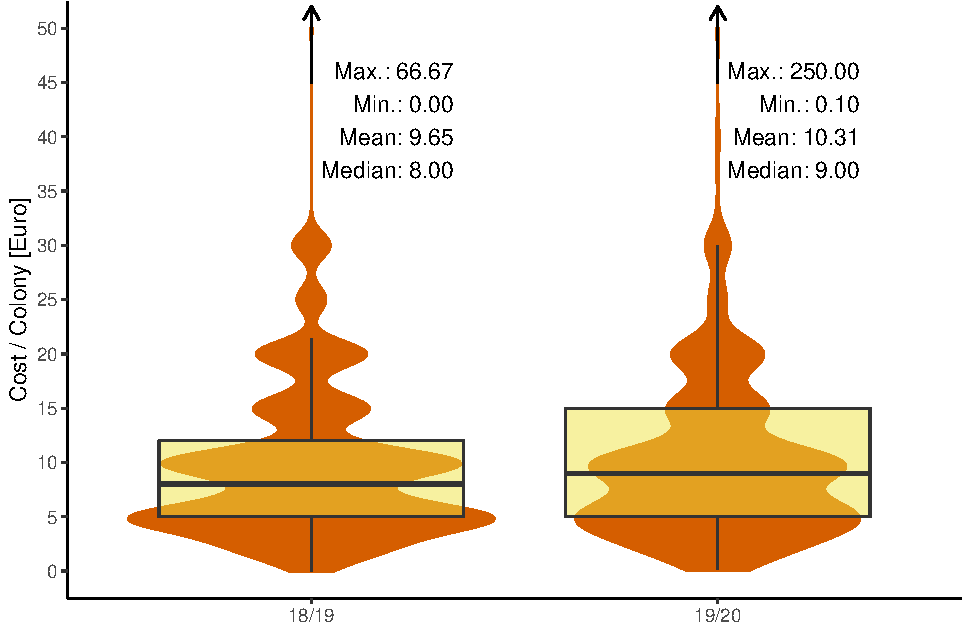
\includegraphics[width=0.8\textwidth]{img/distr-year-1.pdf}
      \caption{Distribution of costs as violin plot in combination with a boxplot. Plot is cutoff at 50.00 Euro.}
      \end{figure}
      \end{minipage}
    \end{block}
    
    {
      \setbeamercolor*{block title}{fg=taaluminium,bg=ta3chameleon}
      \begin{block}{Preemptive Conclusion}
        With our first data exploration we can already see different expenses for different operation size groups. Our estimates which were calculated beforehand are in range with the survey expenses. It seems the question in the survey was not clear, as many participants did answers the complete expenses and not per colony. Further data cleanup and also comparison of treatment combinations needs to be done.
      \end{block}
    }

  \end{column}
  %%%%%%%%%%%%%
  % 2. Col %%%%
  %%%%%%%%%%%%%
  \begin{column}{0.49\textwidth}

    {
      \setbeamercolor*{block title}{fg=taaluminium,bg=ta3skyblue}
      \begin{block}{(Info Box) Varroa Mite}
      \begin{columns}[t,onlytextwidth]
        \begin{column}[t]{.5\linewidth}
        \begin{minipage}[t][17.5cm][c]{0.97\textwidth} 
        The parasitic mite \textit{Varroa destructor} is the most important bee pest worldwide and has been widespread in Austria since the 1980s. An active treatment against this parasite is still unavoidable in order to become a successful beekeeper due to the lack of adaptation of our domestic honeybee. The parasitic mite is found mainly in the brood and there preferable in the drone brood \citep{rosenkranz2010}. The mite feeds primarily on the fat body of larvae and adult bees, which are used as phoretic transport medium \citep{ramsey2019}. In the fight against high winter honeybee colony losses, the treatment against the varroa mite plays an important, if not the central role. The parasite has a great influence on the overwintering success of bee colonies \citep{dahle2010}, especially because the mite serves as a vector for other pathogens, such as viruses \citep{rosenkranz2010, noel2020}. \\
        In Austria most beekeepers use a combination of organic acids to treat their colonies against the varroa mite \citep{moosbeckhofer2015, oberreiter2020}. 
        \end{minipage}
        \end{column}
        \begin{column}[t]{.5\linewidth}
        \begin{figure}
        \centering
        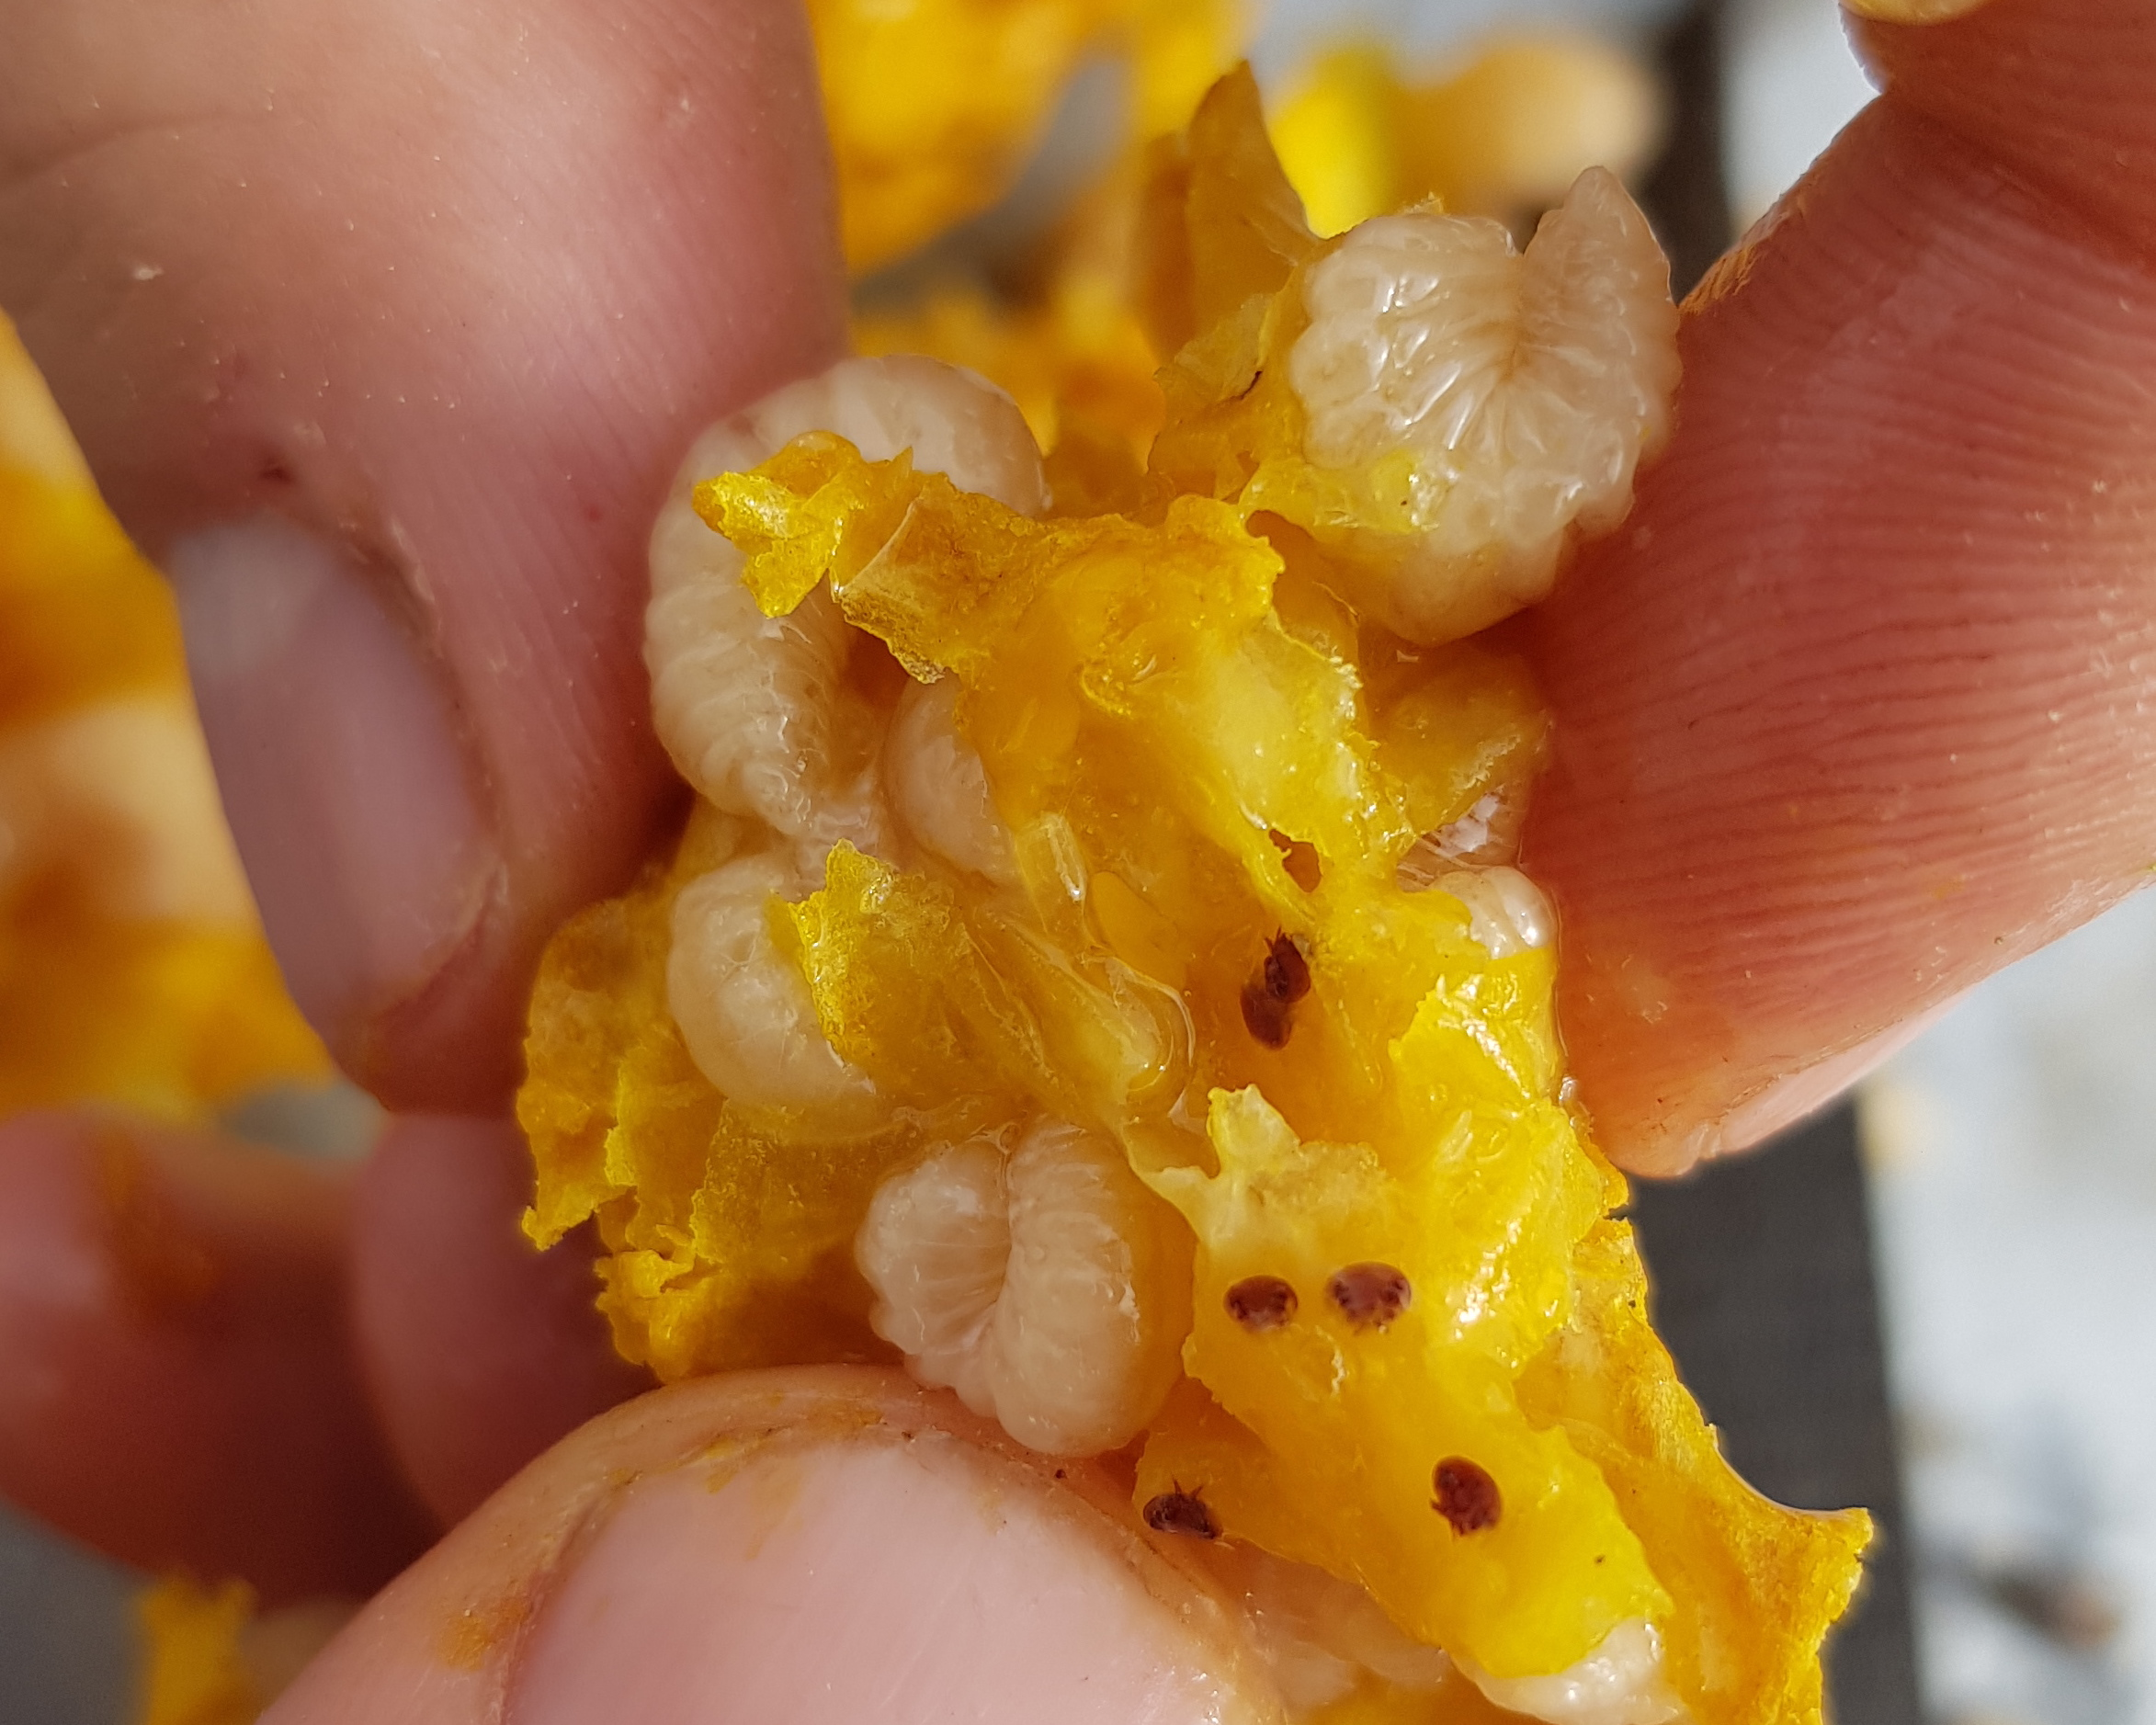
\includegraphics[width=0.8\textwidth]{img/varroa.jpg}
        \caption{Honeybee dronebrood highly invested with Varroa Mites.}
        \end{figure}
        \end{column}
      \end{columns}
      \end{block}
    }

    {
      \setbeamercolor*{caption name}{fg=ta2aluminium}
      \setbeamercolor*{caption}{fg=ta2aluminium}
      \begin{figure} 
      \begin{minipage}[t][0.15\paperheight][c]{0.97\textwidth} 
      \vskip-\baselineskip
      \centering
      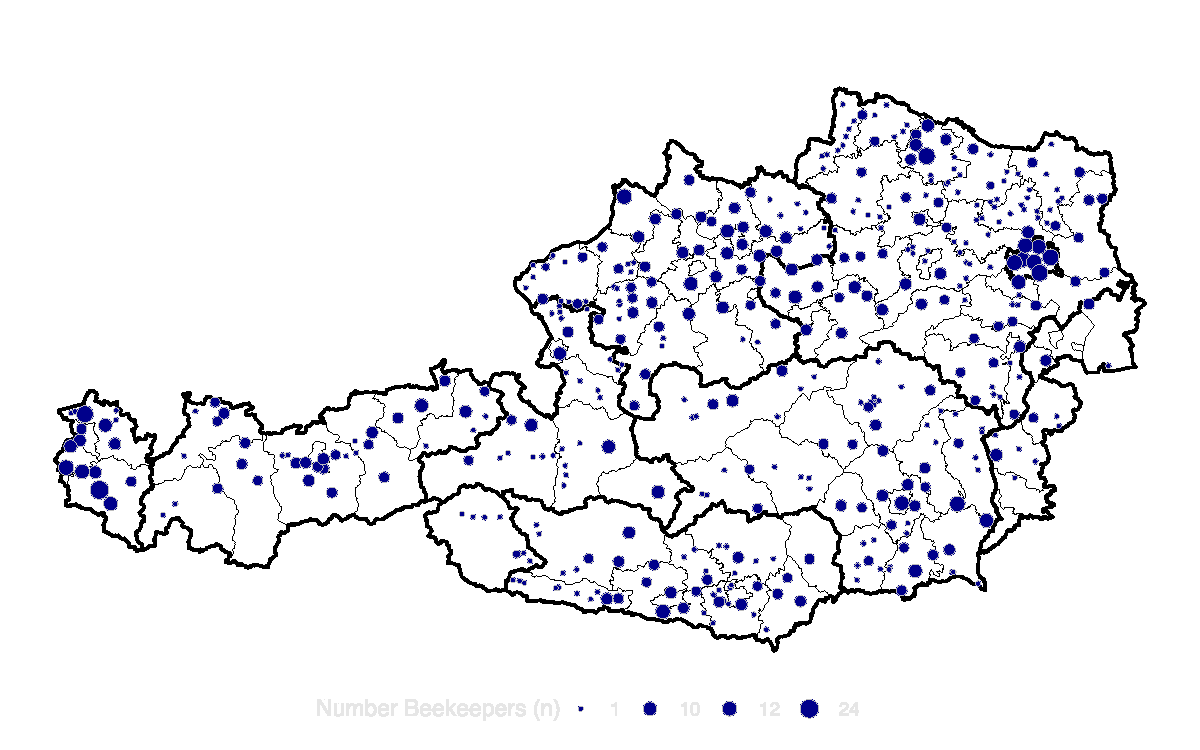
\includegraphics[width=.65\textwidth]{img/plot_overview_map2.pdf}
      \caption{The approximate location of the main winter apiary showed a nationwide coverage all over Austria from the 2019/20 survey. Shapefiles under \enquote{Creative Commons}: \url{https://www.data.gv.at/}}
      \end{minipage}
      \end{figure}
      \vspace{0.5cm}
    }

    \begin{block}{Expenses Estimations}
      \begin{figure}
      \begin{minipage}[t][0.20\paperheight][c]{0.97\textwidth} 
      \centering
      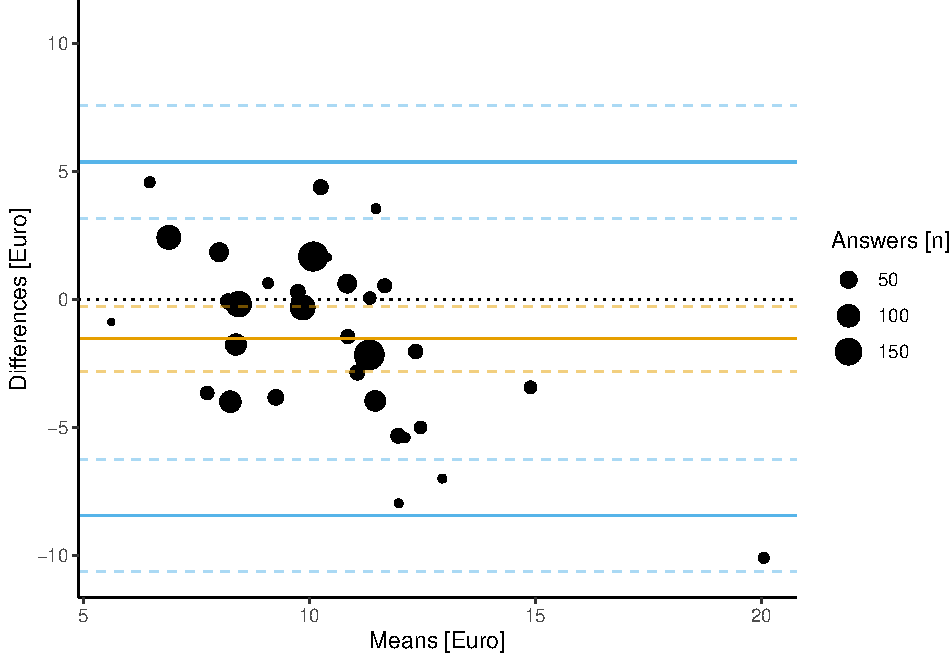
\includegraphics[width=0.8\textwidth]{img/estimates-bland-1.pdf}
      \caption{Analysing of our calculated estimates with the survey results for common treatment methods was done with Bland-Altman plot. Blue horizontal lines indicating 95\% CI and orange line represents the mean difference. We can observe that most combinations are inside our defined CI, but survey is expenses on average below our calculated estimates}
      \end{minipage}
      \end{figure}
    \end{block}

    \begin{block}{Operation Size}
      \begin{figure}
      \begin{minipage}[t][0.20\paperheight][c]{0.97\textwidth} 
      \centering
      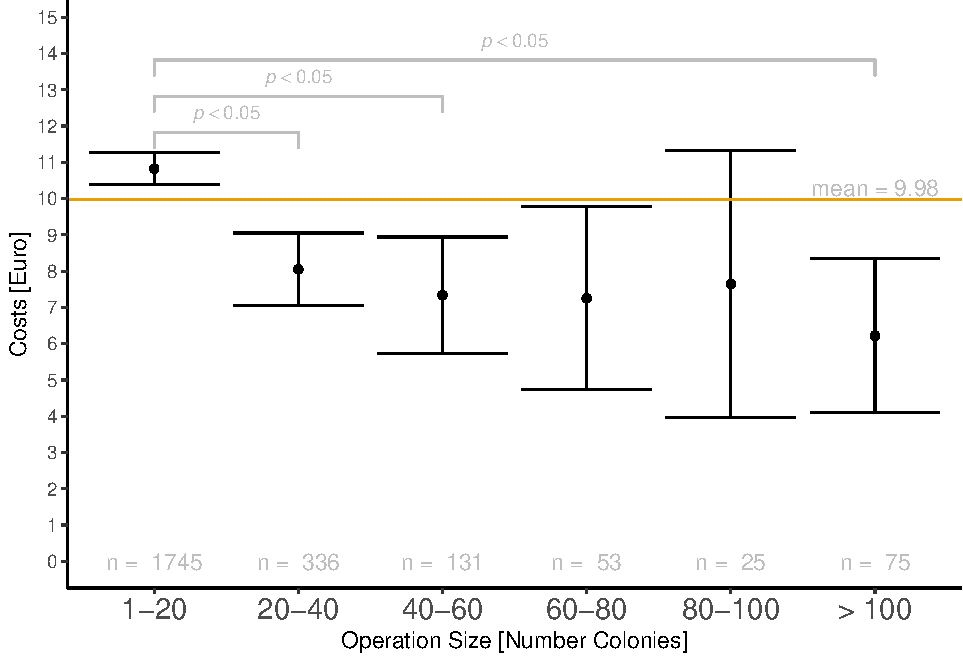
\includegraphics[width=0.8\textwidth]{img/operation-ci-1.pdf}
      \caption{To compare different operation size groups, we used the number of hives wintered from the survey to group the beekeepers in their respective operation size group. Confidence intervalls were generated with GLM (formular: $Cost \sim 0 + Operation Size$), significant test with pairwise t-test and family-wise error corrected $p$-value (Holm, Step Down).}
      \end{minipage}
      \end{figure}
    \end{block}


    {
      \setbeamercolor*{block title}{fg=taaluminium,bg=gray}
      \setbeamercolor*{block body}{fg=white,bg=black}
      \begin{block}{References}
      {
      \footnotesize
      \printbibliography
      }
      \end{block}
    }

  \end{column}
\end{columns}

%\vfill
\end{frame}
\end{document}